\section{Design Parameterization and Processing Pipeline}

Figure~\ref{fig:model_training_pipeline} summarizes the processing path used to move from canonical optical prescriptions to model-facing training tables and back to simulation-ready generated designs. The key design choice is to keep a single canonical prescription table as the dataset reference, then derive representation-specific tables for generative modeling. This separates optical data definition from model-specific formatting choices such as normalization, imputation, and file layout.

\begin{figure}[ht]
    \centering
    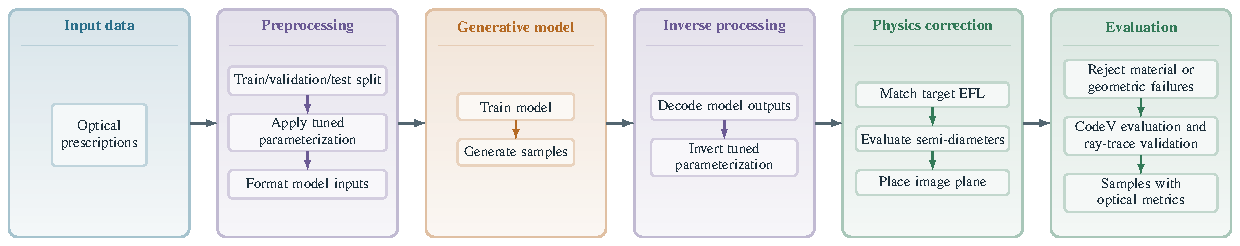
\includegraphics[width=\linewidth]{figures/model_processing_pipeline_filled_tikz.pdf}
    \caption{\textbf{Model-facing data and post-processing pipeline.} Optical prescriptions are partitioned, mapped into the tuned parameterization, formatted for model input, generated, and decoded. The inverse transform restores physical parameters before physics correction. Material or geometric failures are rejected before CodeV evaluation; successful ray traces provide optical metrics. Colors denote input data (teal), reversible deterministic transformations (purple), learned generation (orange), and optical correction and evaluation (green); arrows indicate forward data flow.}
    \label{fig:model_training_pipeline}
\end{figure}

\subsection{Canonical Table and Model-Facing Representations}
\label{sec:canonical_model_representations}

The canonical table stores each optical prescription in the common tabular schema introduced in the dataset section and detailed in Appendix~\ref{app:dataset_details}: surface geometry, material assignment, topology, design conditions, field and wavelength setup, optical-performance annotations, and provenance. Model-facing data are derived from this canonical table after separating prescription and design-condition variables from provenance columns, filtering flags, and optical-performance columns. The generative models are therefore trained on optical prescriptions and design conditions, not on the measured performance values that are reserved for evaluation.

We use two representation families. The \emph{untuned} representation keeps curvature, thickness, semi-diameter, and stop variables close to their canonical physical form and serves as the direct tabular baseline. The \emph{tuned} representation expresses curvature relative to system length, valid thicknesses as axial fractions with explicit system-length terms, semi-diameter relative to entrance-pupil diameter, and stop location relative to surface count. Both representations use continuous material-property coordinates with an explicit air indicator, preserve the same row order and split labels, and apply the same structural missingness mask. Appendix Table~\ref{tab:tuned_untuned_representation} provides the complete variable-by-variable comparison and inverse-processing rules.

For both representations, the material labels used for CodeV export are reconstructed after generation from the generated material variables. If a surface is marked as air, the air indicator takes priority over generated $N_d$ and $V_d$ values. Otherwise, generated material properties are projected to the nearest available catalog material. This keeps material generation continuous during modeling while returning to discrete material labels for optical simulation.

\subsection{Variable Surface Count and Structural Missingness}

Lens prescriptions have variable surface count, but the tabular benchmark models require a fixed column set. We therefore reserve surface-indexed columns up to the maximum supported surface count and use structural missing values for inactive surface slots. These missing values are not ordinary data gaps: they indicate that the corresponding surface does not exist for that design. During preprocessing, missing values inside active surface slots are treated as data-quality errors, while missing values outside the active surface count are preserved as structural padding. During post-processing, generated samples are re-masked using their generated surface count so that inactive surface slots remain empty before export.

The common representation layer also preserves row identity and split information, and writes provenance and performance information into sidecar artifacts rather than mixing them into the model-facing feature matrix. This makes the model-facing inputs and split assignments auditable without asking the generative model to learn source-folder, lineage, or performance-metric fields.

\subsection{Model-Specific Formatting and Normalization}

The common representation layer stops before model-specific numerical formatting. This is important for fair benchmarking: TabSyn, STaSY, CoDi, and other baselines can use the normalization, imputation, and mixed-type encodings required by their own training code, while starting from the same untuned or tuned optical representation. For example, quantile normalization is not part of the common representation definition; it is applied only when required by a particular benchmark implementation. This separation prevents model-specific preprocessing from being mistaken for an optical representation change.

\subsection{Generated-Sample Inverse Processing}

Generated samples are mapped back to canonical-style prescription tables before simulation. The inverse processor applies the paired inverse of the representation transform, restores deterministic field and wavelength defaults used by the canonical schema, reconstructs material labels from generated material variables, and re-applies the structural surface mask implied by the generated surface count. For generated rows, provenance sidecars from the training data are not copied row-by-row; only deterministic schema defaults and values inferable from the generated prescription are restored. This distinction is necessary because a generated batch does not share the row identity of the original training table.

\subsection{Physics-Based Post-Processing}

After inverse processing, generated prescriptions in the finalized pipeline pass through a ray-tracing-based correction layer before CodeV evaluation. This layer makes local optical corrections to the generated prescription rather than defining the training representation. The controlled ablation in Section~\ref{sec:results_raytrace_postproc} evaluates the same generated rows without this layer to isolate its contribution. The correction attempts the following stages:

\begin{enumerate}
    \item \textbf{Material and geometry precheck}: verify that active surfaces have valid material and geometry information before ray tracing is attempted.
    \item \textbf{Final-surface curvature tuning}: adjust the final active surface curvature to better match the generated target effective focal length using first-order ray-tracing estimates.
    \item \textbf{Semi-diameter evaluation}: recompute active-surface semi-diameters from traced rays while checking for geometric inconsistencies.
    \item \textbf{Image-plane placement}: adjust the final image gap using the traced focal location.
\end{enumerate}

The correction is applied stage by stage: a successful earlier correction can be retained even if a later correction is not available for a particular sample. Stage outcomes are recorded so that evaluation can compare generated prescriptions before and after ray-tracing correction using a common denominator.

\subsection{CodeV Preparation}

The final post-processed table is prepared as a CodeV-ready prescription table with canonical field, wavelength, material, surface, and image-plane columns. Sequence-file generation and CodeV execution are handled by the downstream simulation pipeline. This keeps the generative-model pipeline responsible for producing simulation-ready prescription tables, while the optical simulation pipeline remains responsible for generating sequence files, running CodeV, and returning optical-performance results.
